\section{Appendix}

This is where you can include your documentation.

Remember that the marker is not required to read this, but might well check to ensure that you have included product documentation, and ethical approval, as required.
\subsection{Tests}
The following are all the aspects of the app that the JEST tests cover.
\begin{itemize}
  \item The Analysis component renders correctly with default settings
  \item The Analysis component renders without errors
  \item Verifies that the element with the test ID analysis-container is present in the rendered output of the Analysis Screen component
  \item Ensures the Calendar component renders without errors
  \item Verifies that the Calendar component is displayed correctly with the current month and year
  \item Navigates to the previous month when the left button (<) is pressed in the Aalendar component
  \item Navigates to the next month when the right button (>) is pressed in the Aalendar component
  \item Ensures the Home component renders without errors
  \item Verifies that the text ``Symptoms'' and ``Period'' are present in the rendered output
  \item Ensures the Learn component renders without errors
  \item Verifies that the tab buttons ``For You'' ``Recent'' ``Symptom Relief'' and ``All Articles'' are displayed
  \item Verifies that the Recent tab's font weight changes to bolder indicating it is selected
  \item Correctly filters articles based on the ``symptoms'' keyword
  \item Opens the article URL when an article is pressed
  \item Ensures the MostCommon component renders without errors
  \item Verifies that all common symptoms are displayed with their corresponding severity levels
  \item Ensures the PeriodSquare component renders without errors
  \item Checks that the text style includes fontSize: 15 and color: ``\#009668''
  \item Checks that the text style includes color: 'white' when selected
  \item Ensures the Slider component renders without errors
  \item Renders the Slider component correctly with large text enabled
  \item Ensures the Slider component renders correctly when the highContrast setting is enabled
  \item Renders the Slider component correctly with a specific value
  \item Ensures the TabButton component renders without errors
  \item Renders the Track component correctly
  \item Updates selected period state when a period button is pressed
  \item Saves data when the save button is pressed
  \item Ensures the TwoWeek component renders without errors
  \item Verifies that the element with the test ID date-range is present in the rendered output
\end{itemize}

\subsection{Ethical Approval Form}
\includepdf[pages=-,scale=0.9]{Ethics_form.pdf}
\begin{figure}[h!!]
    \begin{center}
      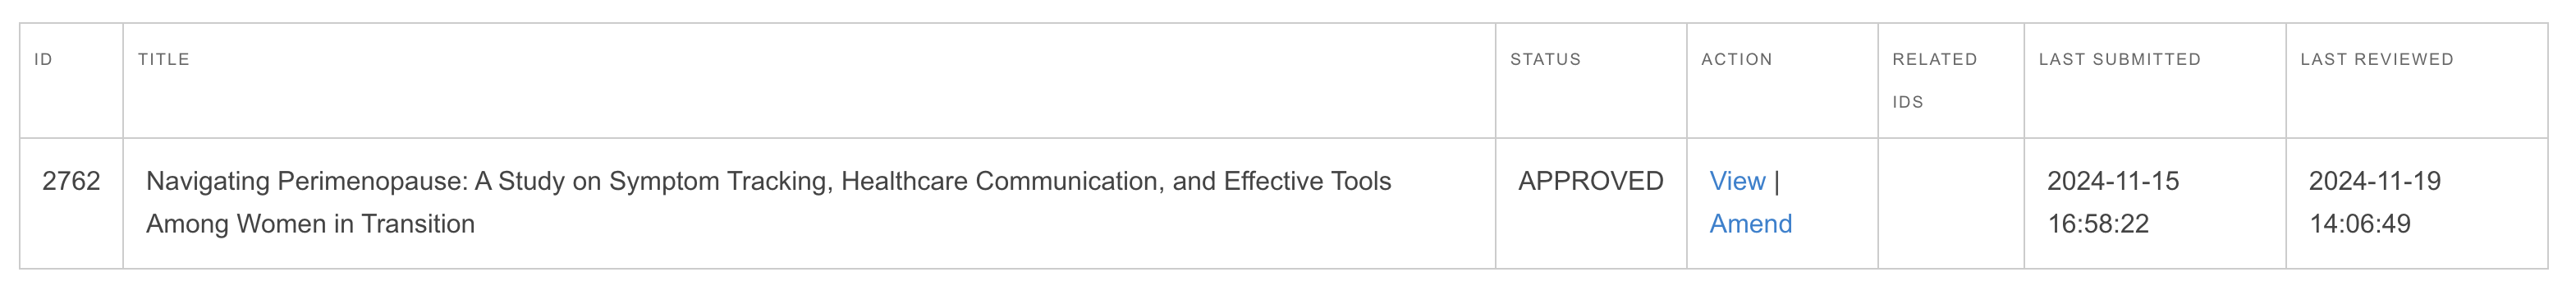
\includegraphics[scale=0.3]{EthicsApproval.png}
      \caption{Ethics Approval.}
      \label{figure:ethics-approval}
    \end{center}
  \end{figure}
  
\subsection{Participant Information Sheet }
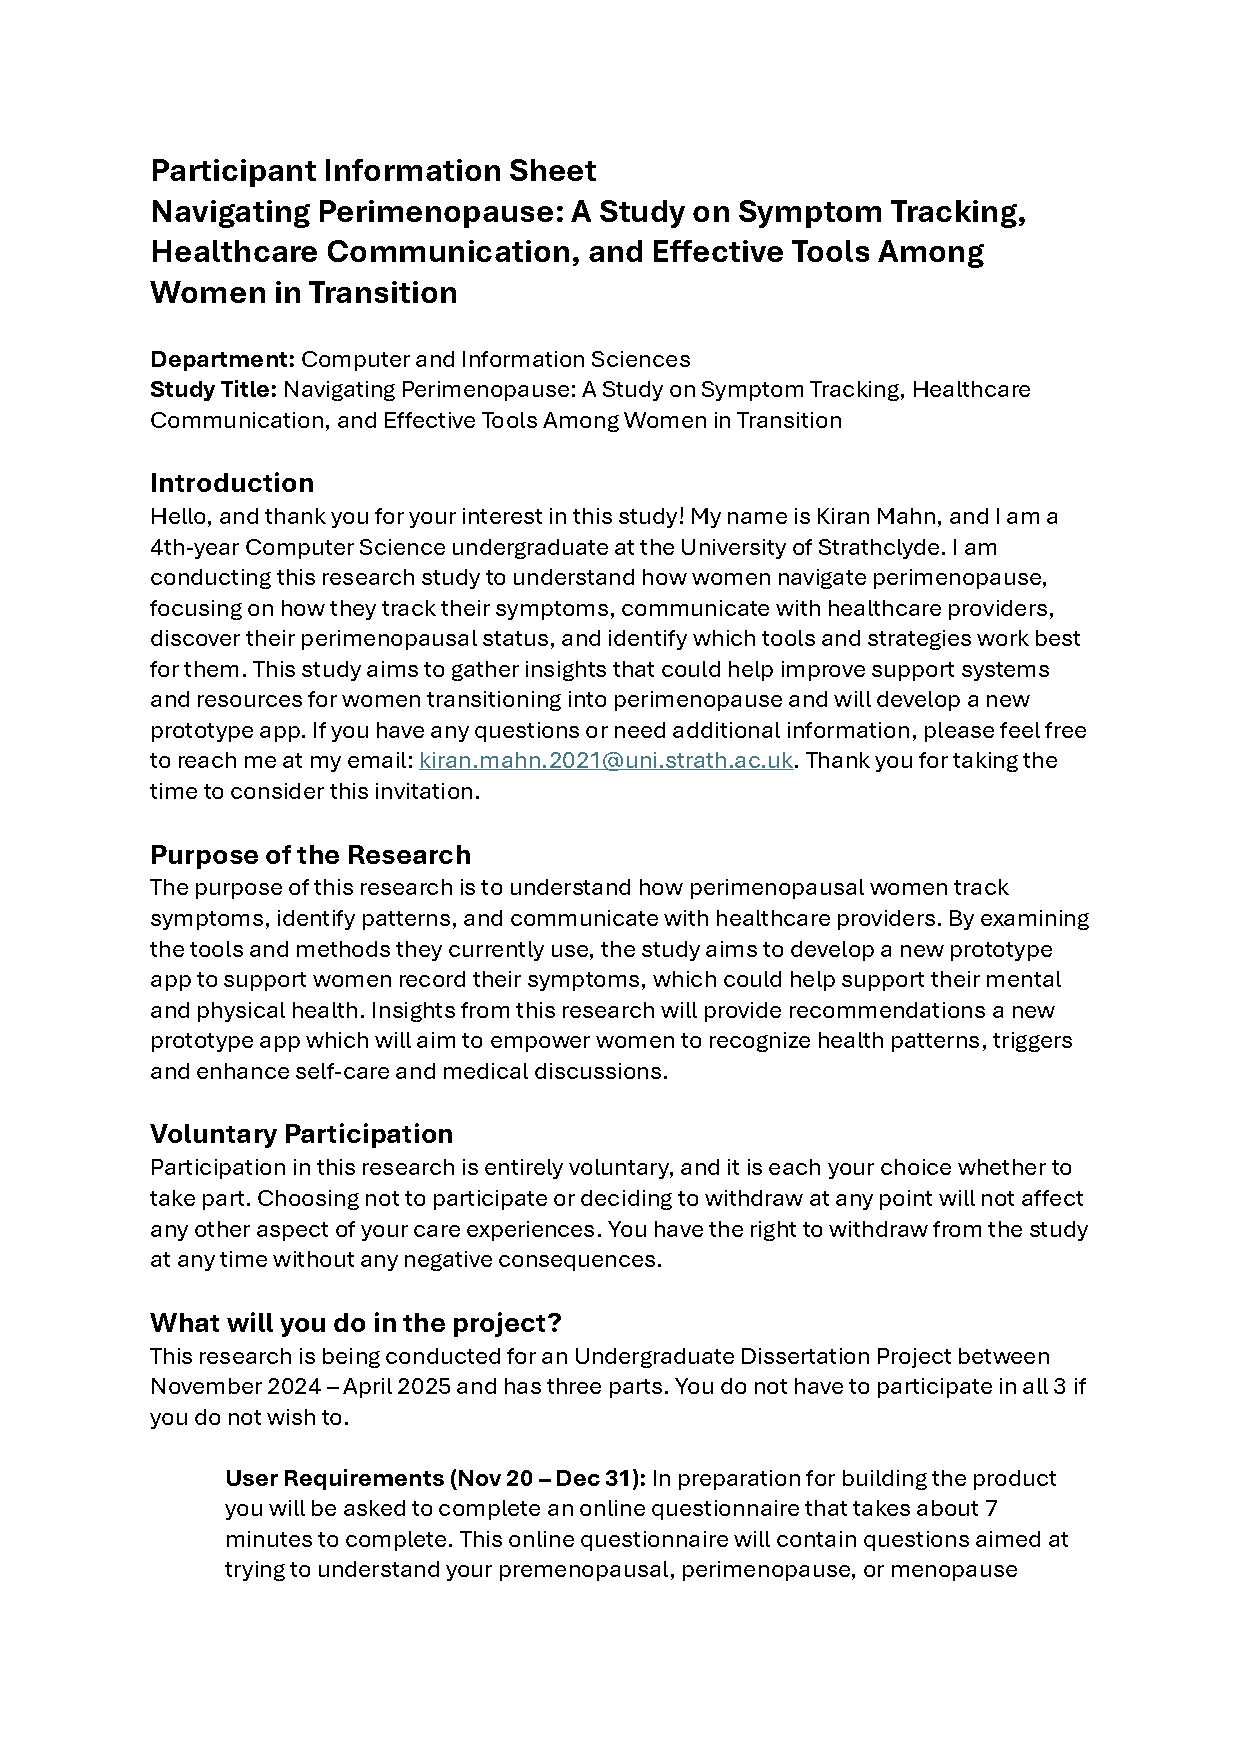
\includepdf[pages=-,scale=0.9]{Participant_Information_Sheet.pdf}

\subsection{Consent Form }
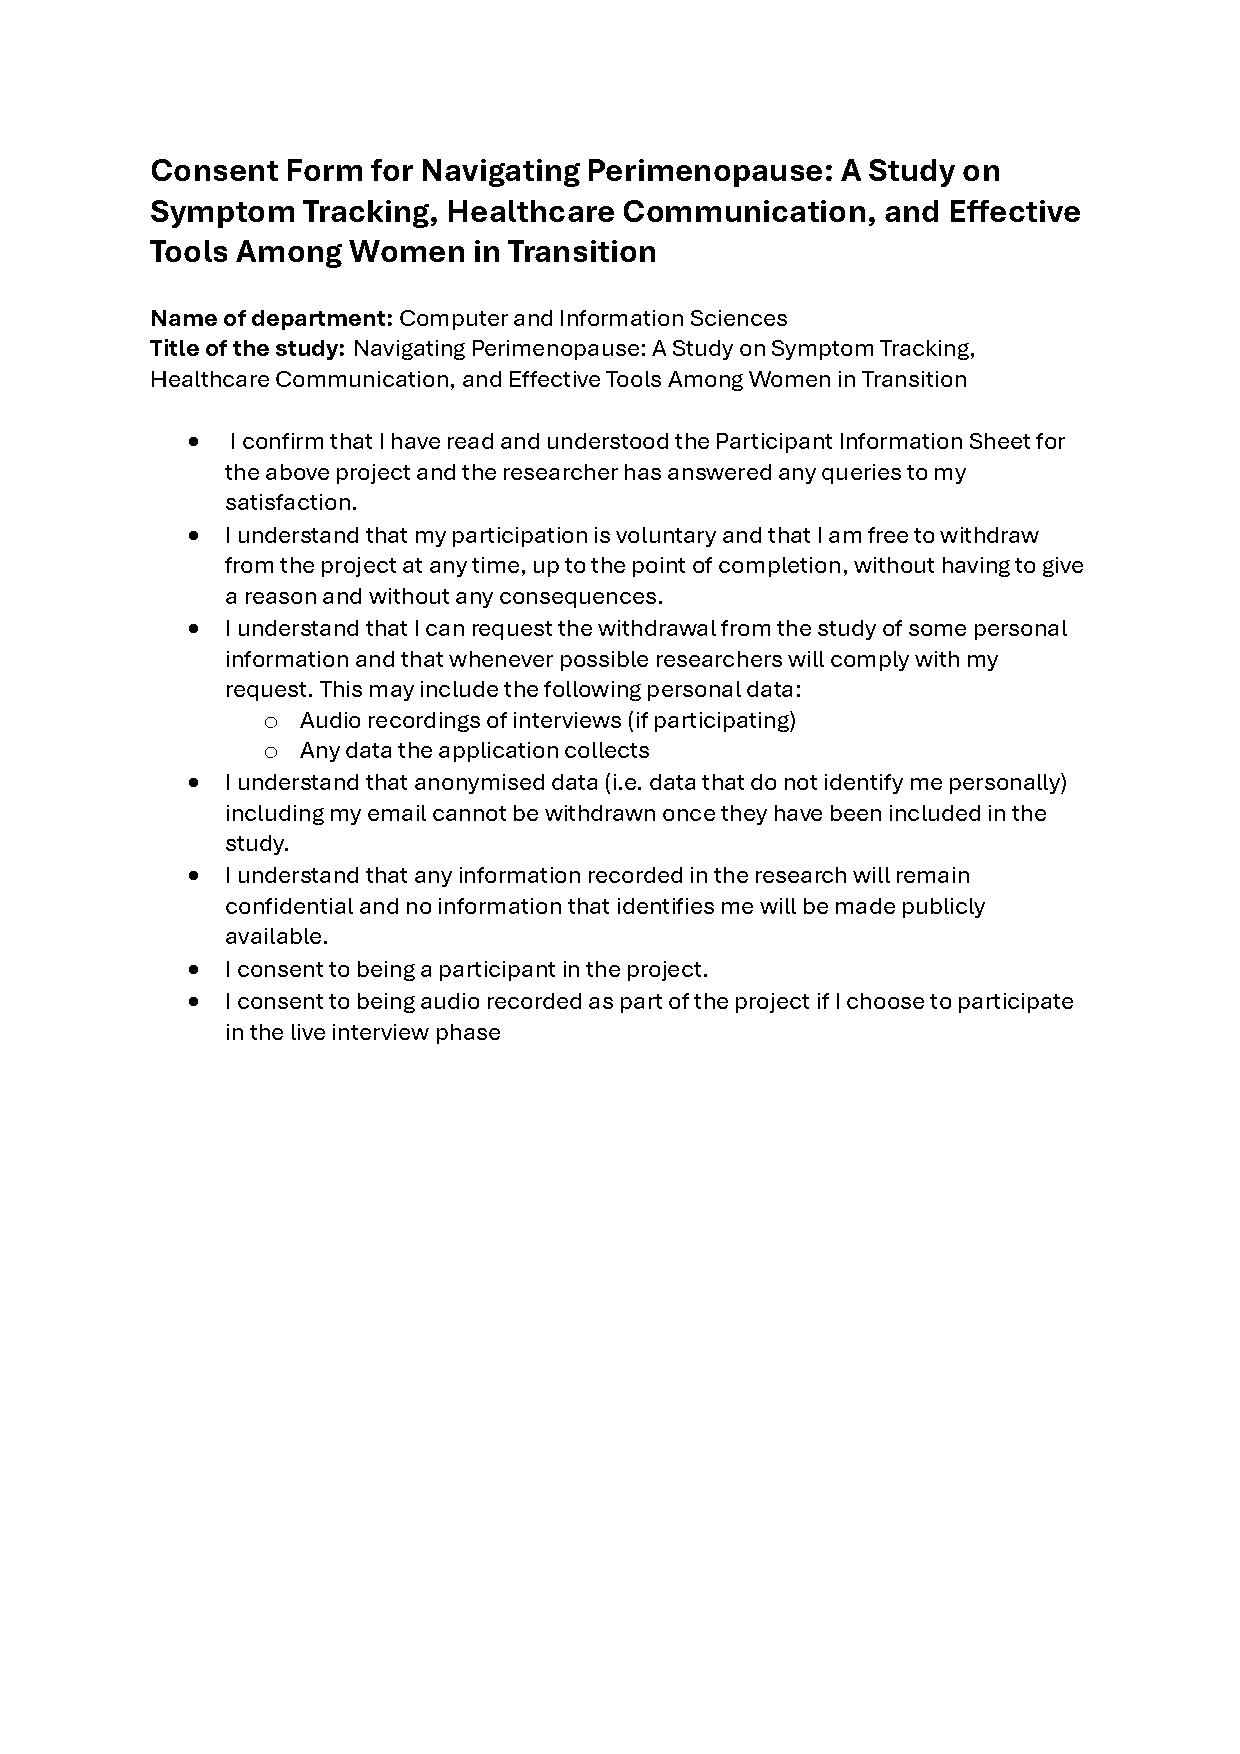
\includepdf[pages=-,scale=0.9]{Consent_Form.pdf}

\subsection{MARS Reviews}
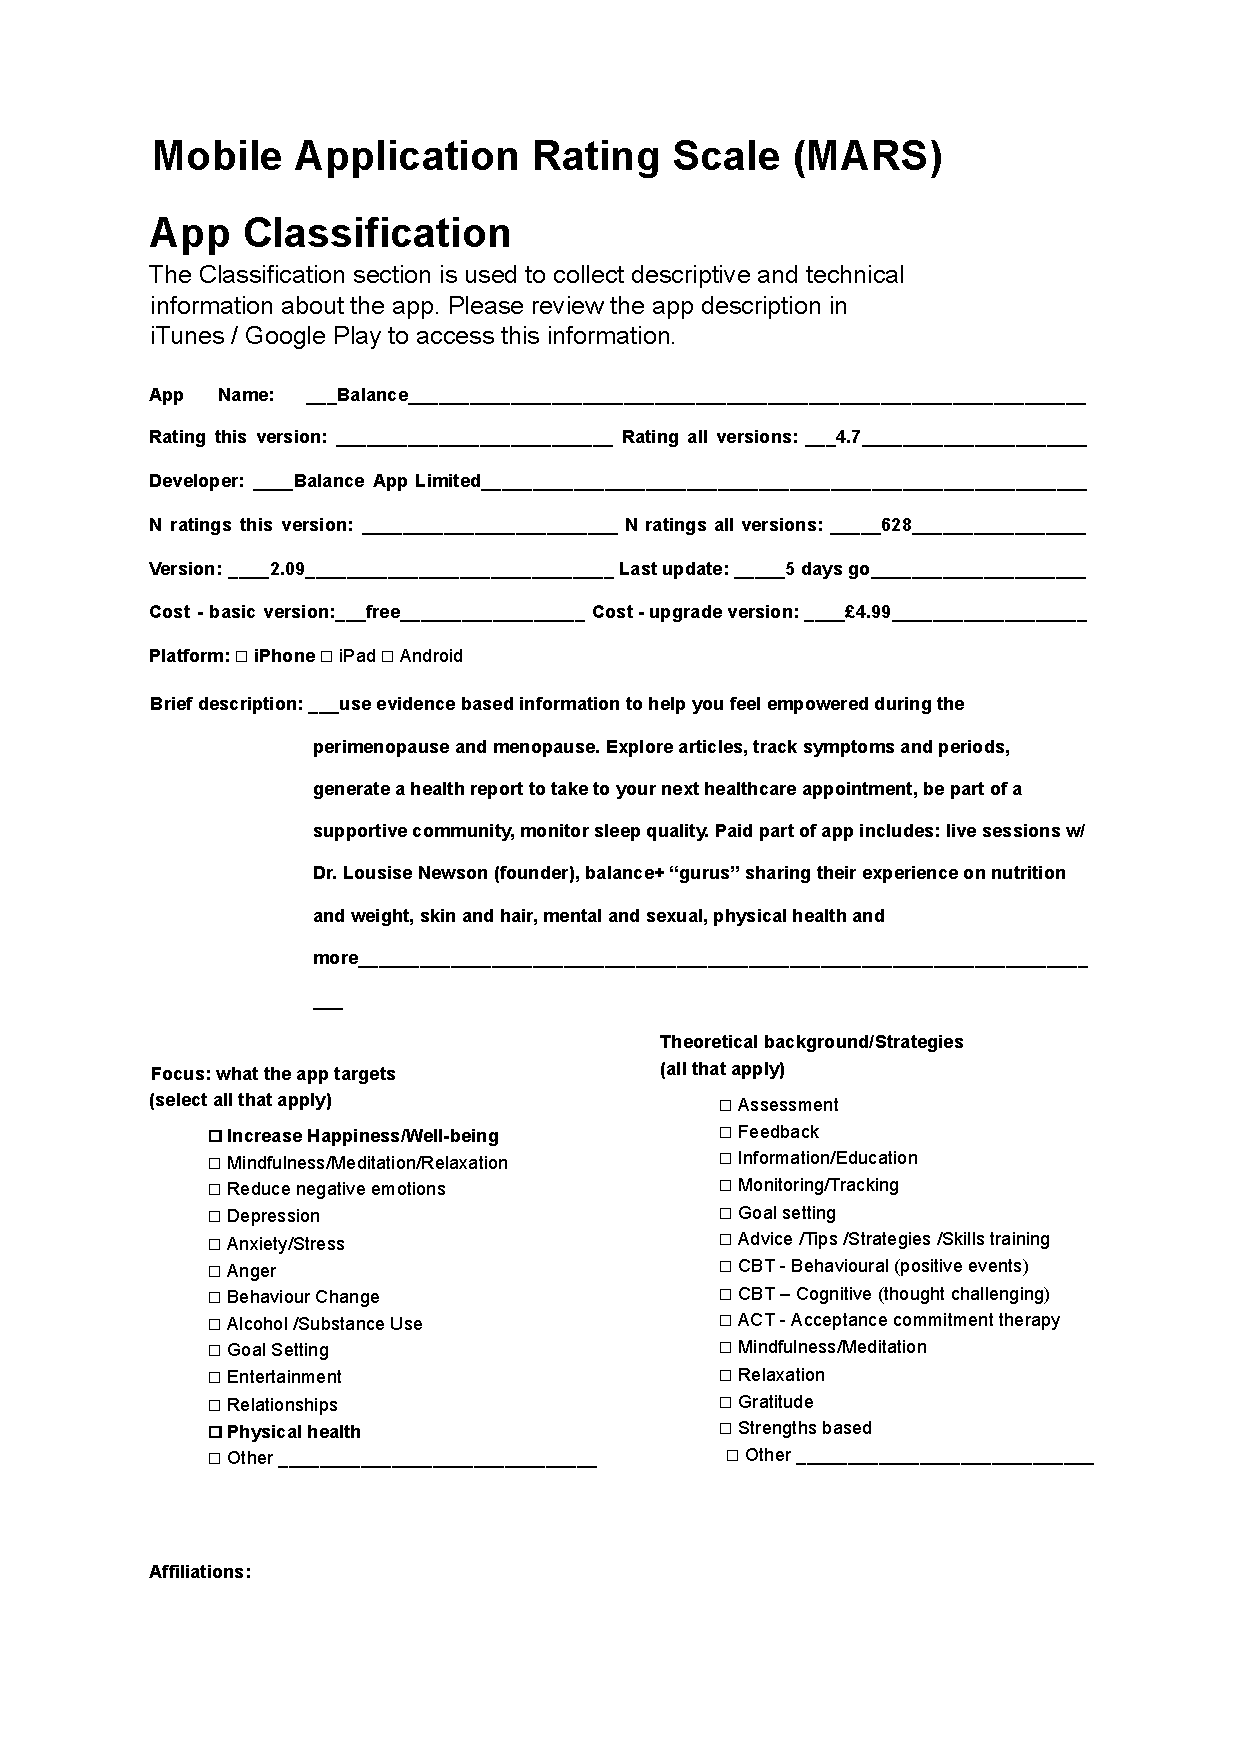
\includepdf[pages=-,scale=0.9]{Balance.pdf}
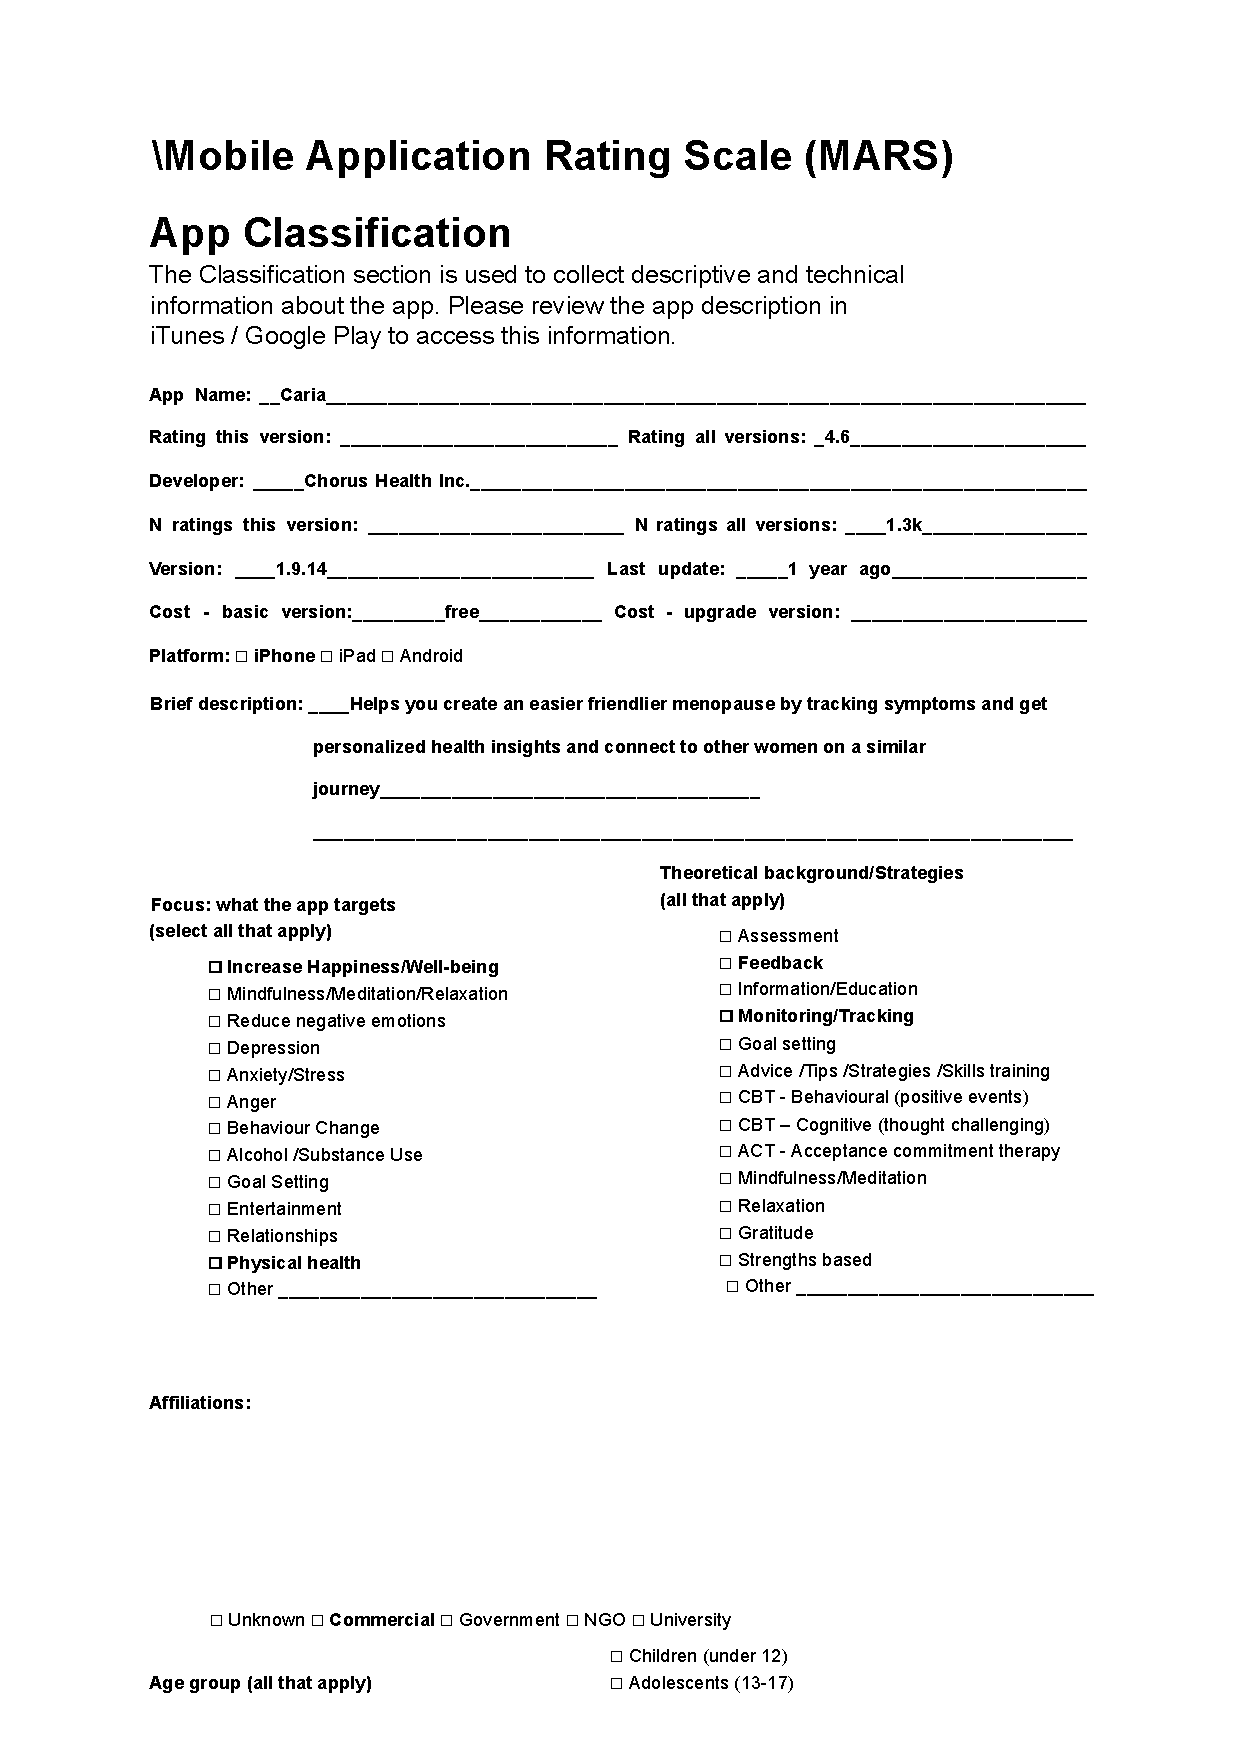
\includepdf[pages=-,scale=0.9]{Caria.pdf}
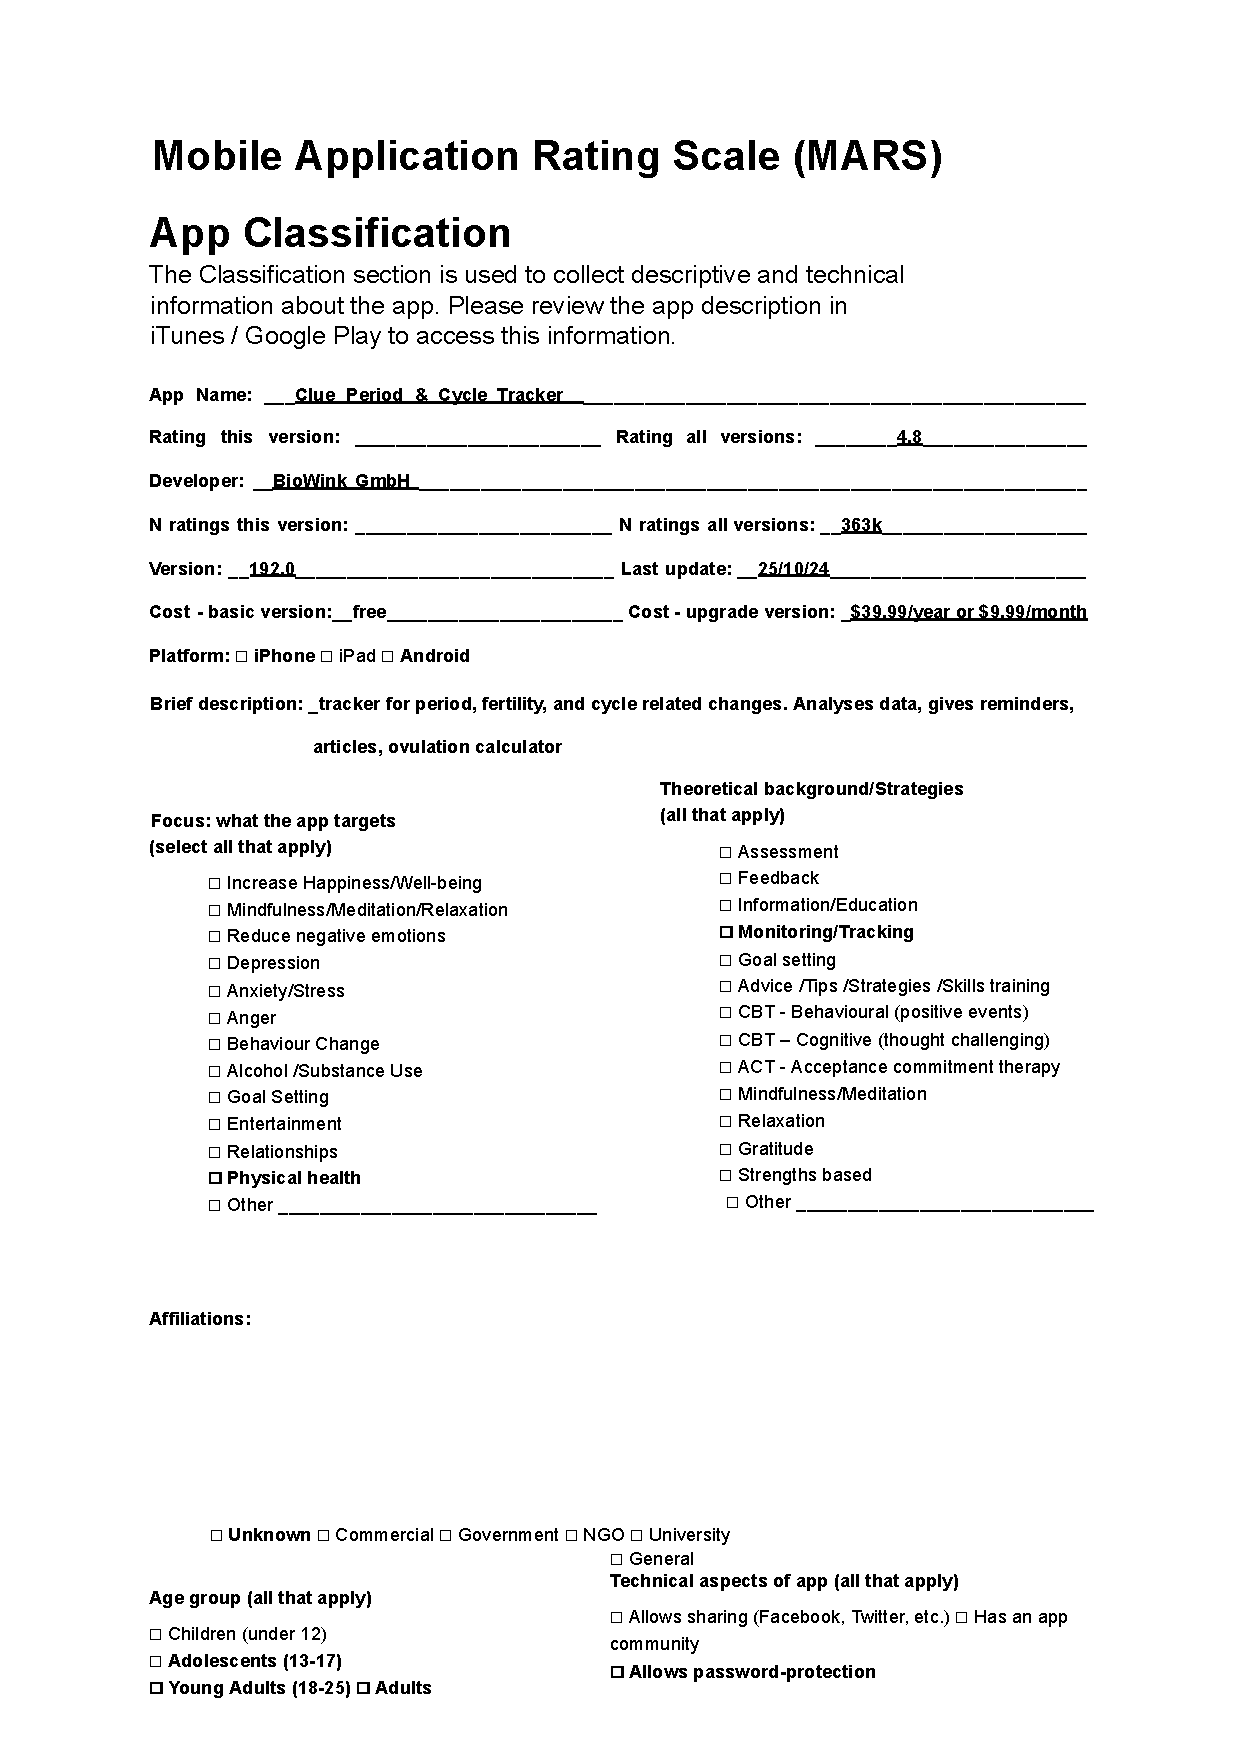
\includepdf[pages=-,scale=0.9]{Clue.pdf}
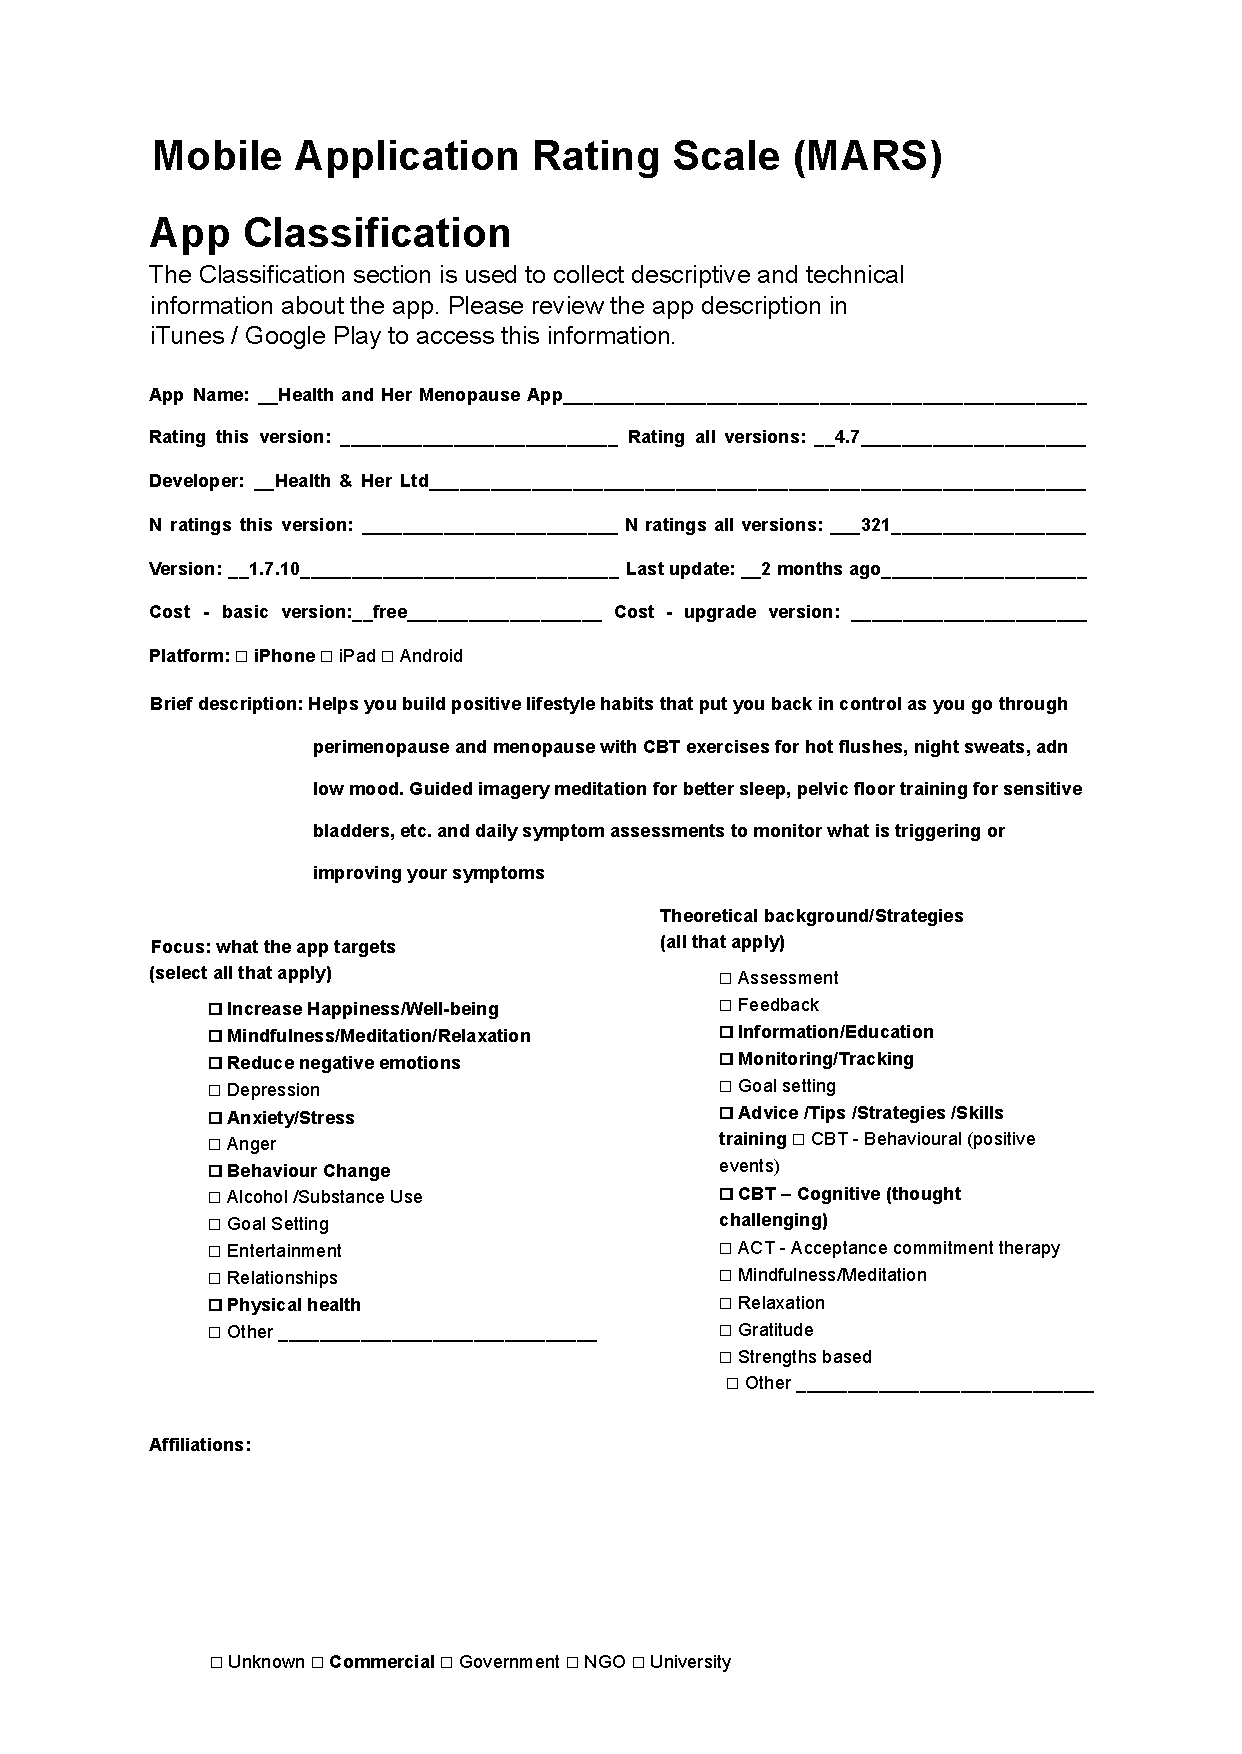
\includepdf[pages=-,scale=0.9]{HealthandHer.pdf}
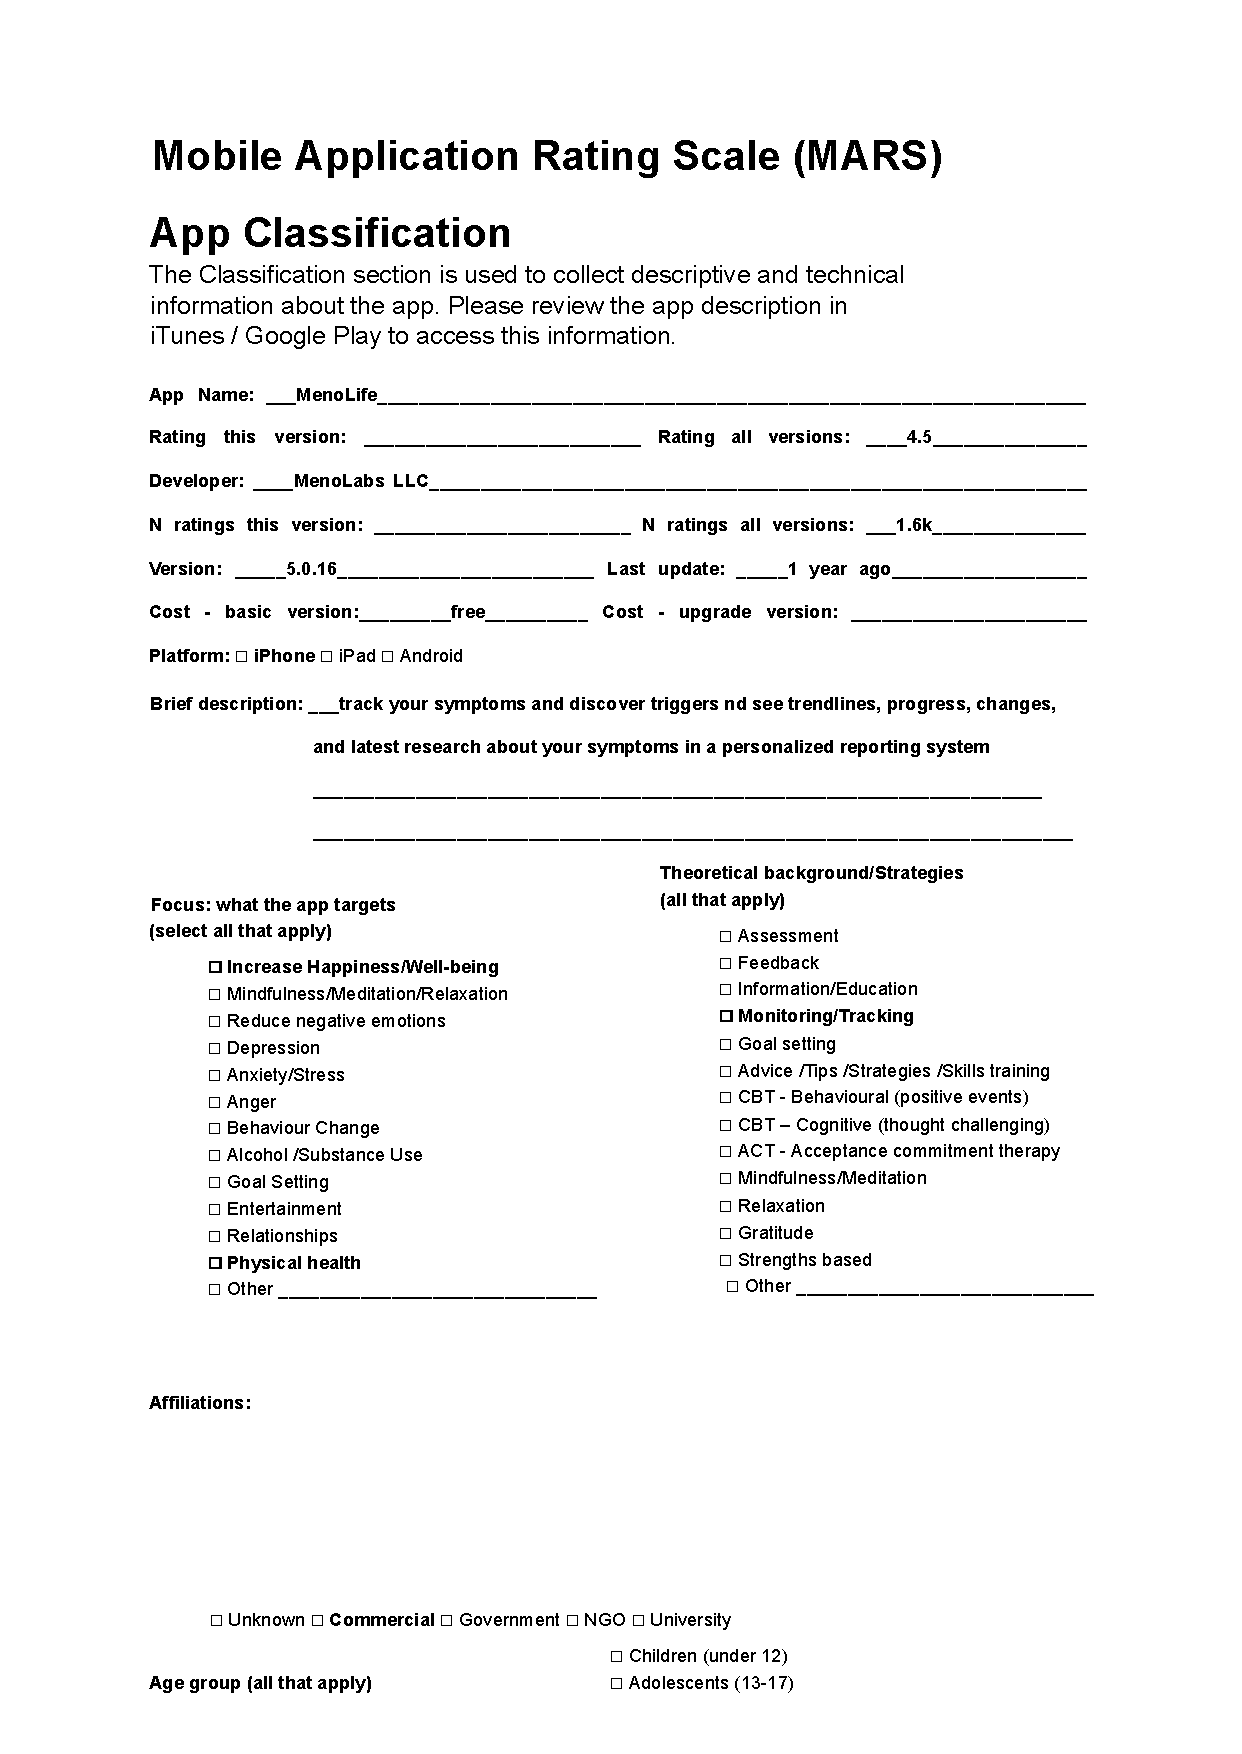
\includepdf[pages=-,scale=0.9]{MenoLife.pdf}
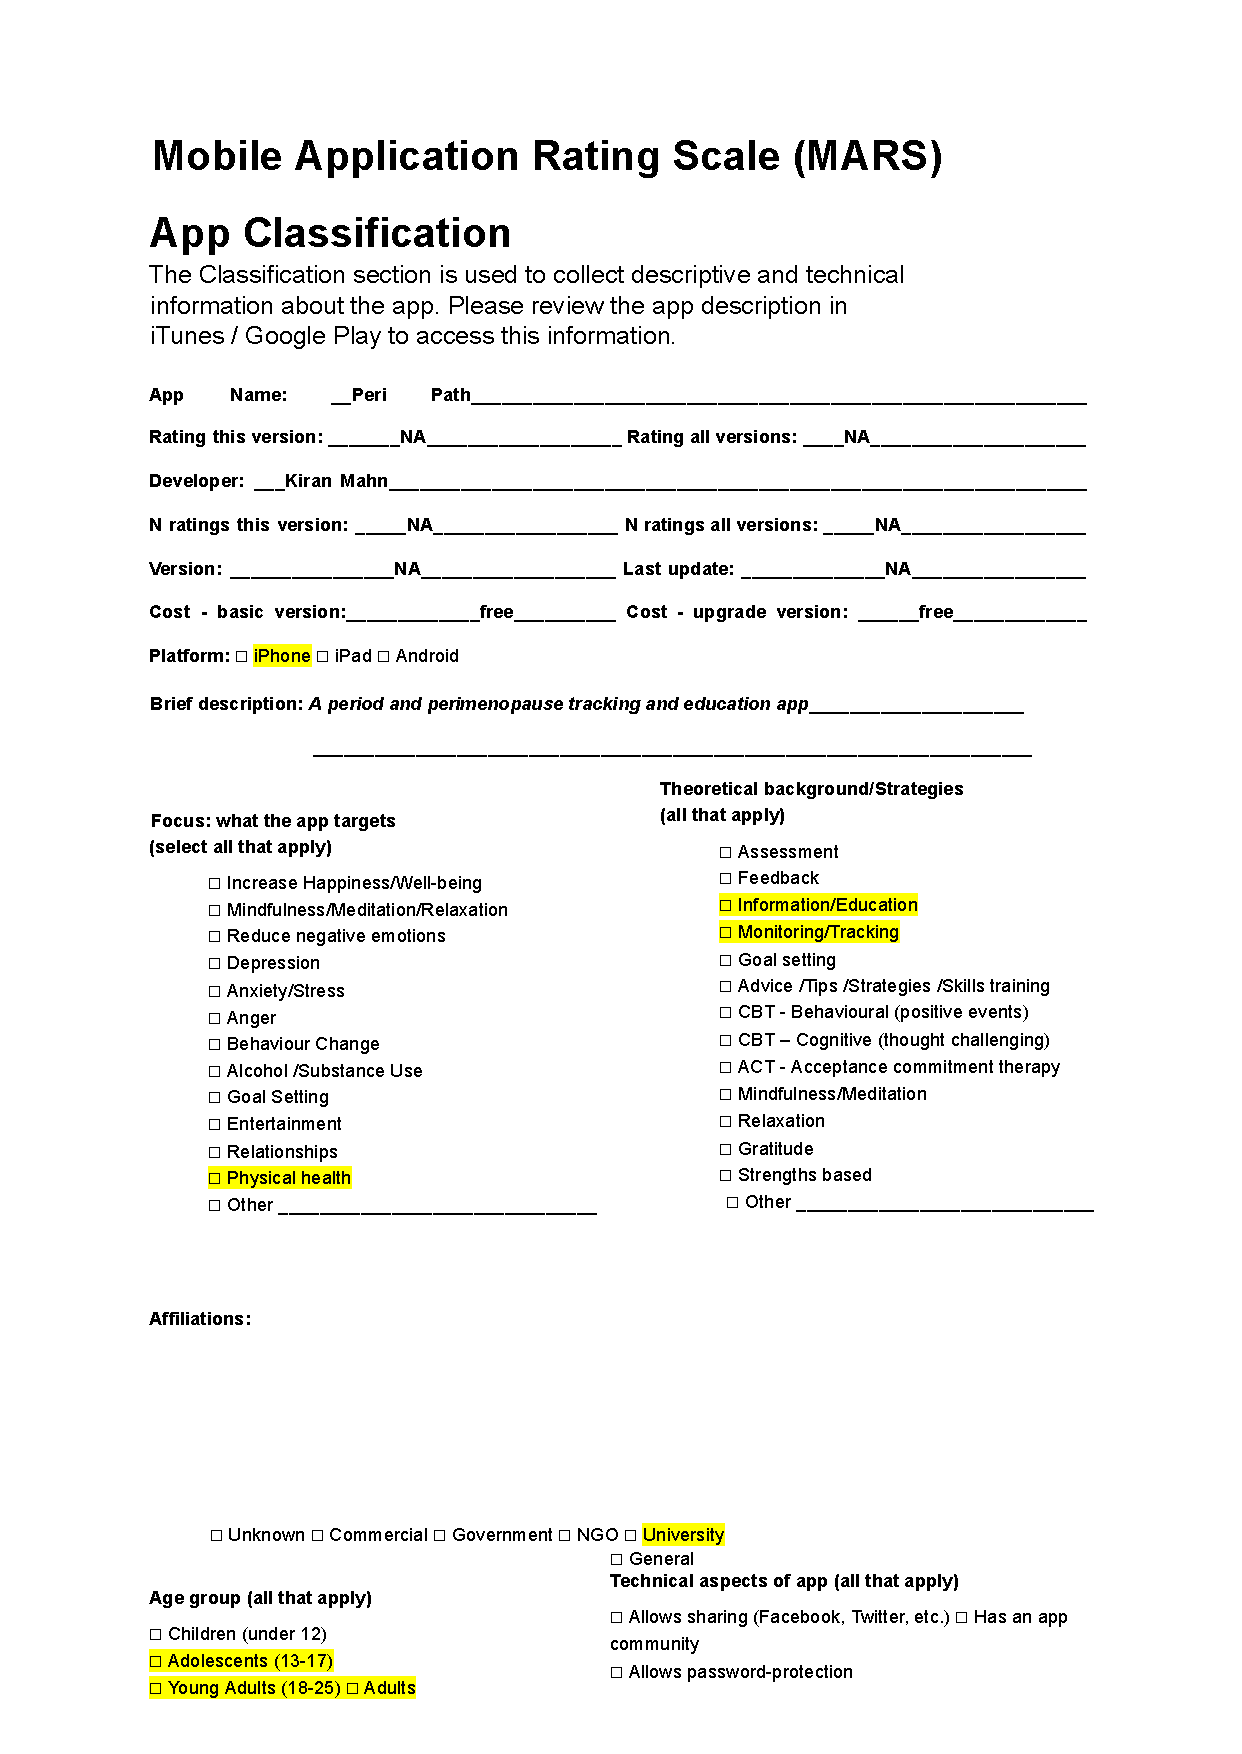
\includepdf[pages=-,scale=0.9]{PeriPath.pdf}
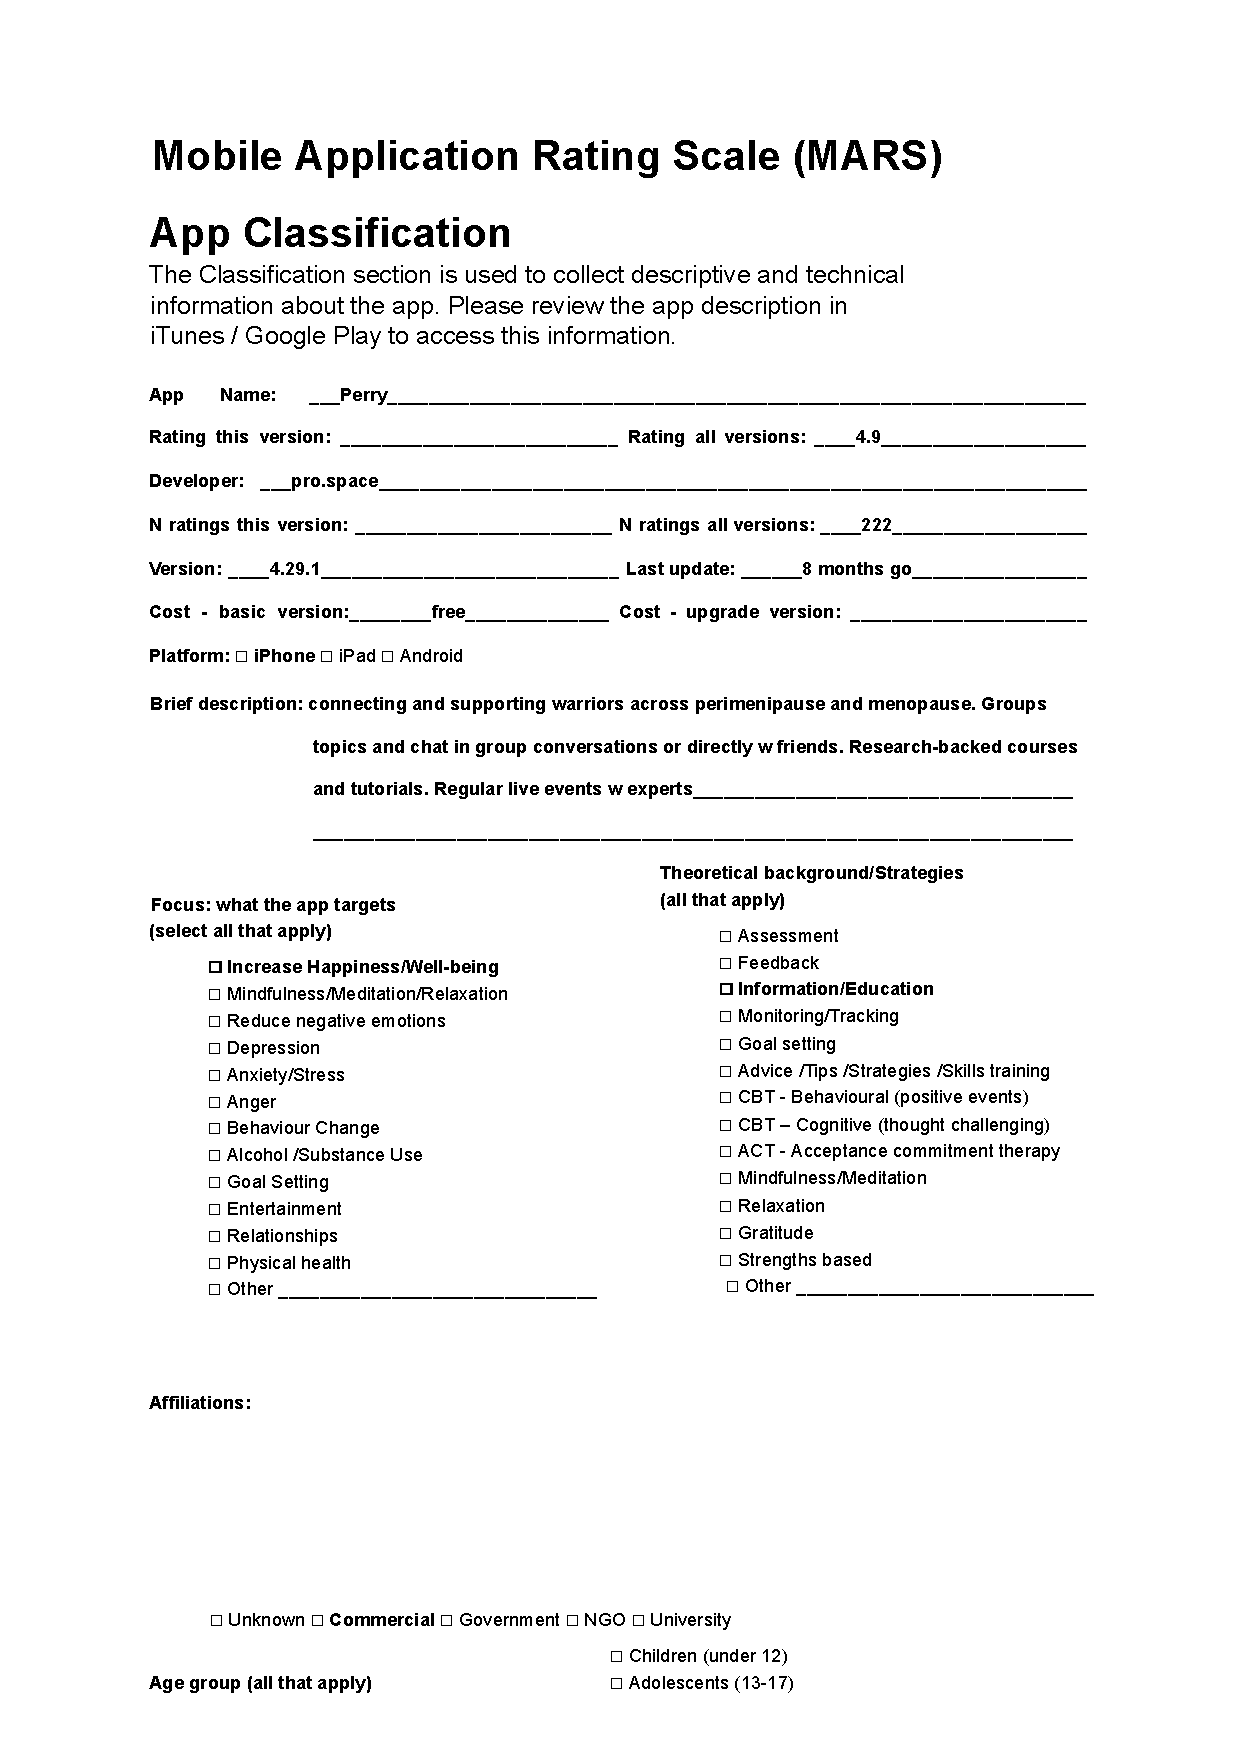
\includepdf[pages=-,scale=0.9]{Perry.pdf}
\includepdf[pages=-,scale=0.9]{OtherMARSEvals.pdf}
\clearpage


 

